\section{Overlay and Cluster Descriptions}

When clustering is complete, each point on the terrain is associated with one of \textit{k} unique clusters. To make this association apparent to the user a cluster overlay is displayed. The clustering overlay attributes a unique color to each cluster and subsequently each terrain vertex a unique color based on cluster membership (see figure \ref{fig:cluster_overlay}). Along with the terrain overlay, a dialogue shows the properties (color, member count, resources) of each cluster (see figure \ref{fig:cluster_dialog}).

\begin{figure}
\center
	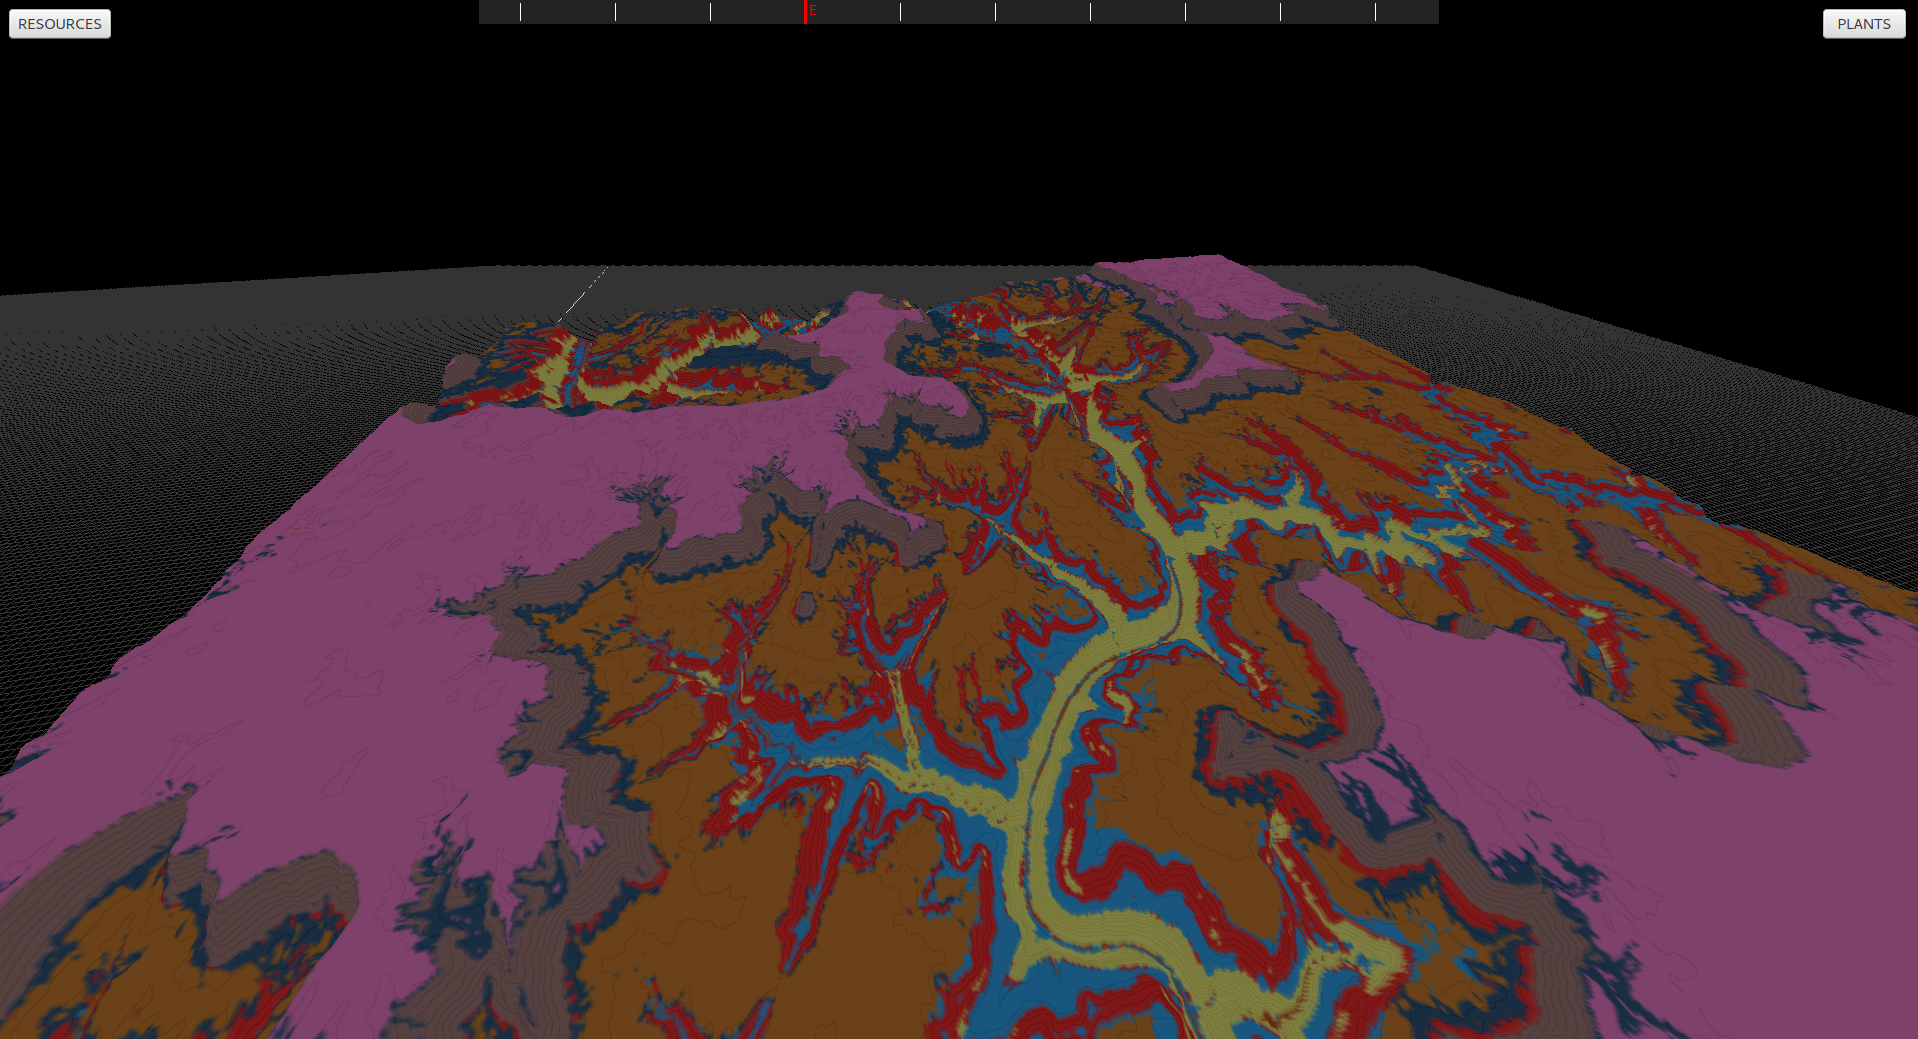
\includegraphics[width=\textwidth]{cluster_overlay.png}
	\caption{ Cluster Overlay. }	
	\label{fig:cluster_overlay}
\end{figure}

\begin{figure}
\center
	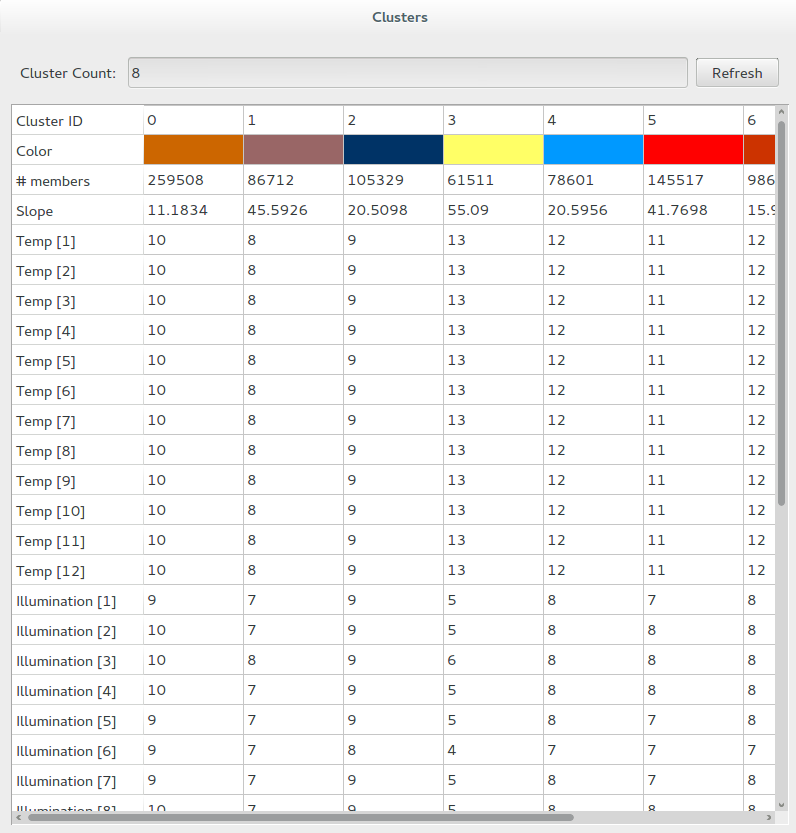
\includegraphics[width=\textwidth/2]{cluster_dialog.png}
	\caption{ Cluster properties dialogue. }	
	\label{fig:cluster_dialog}
\end{figure}

